\documentclass[10pt]{beamer}
\usetheme{Warsaw}
\usefonttheme[onlymath]{serif} 
\setbeamercovered{invisible}
\beamerdefaultoverlayspecification{<+->}

\usepackage[utf8]{inputenc}
\usepackage[english]{babel}
\usepackage[T1]{fontenc}
\usepackage{lmodern,amsmath,booktabs,setspace,mathtools,multicol,url}

\title[Support Vector Machines for Face Recognition...]{Support Vector Machines}
\subtitle{for Face Recognition using \texttt{scikit-learn}}
\author[J Franco Ray]{J Franco Ray \vfill {\footnotesize Scientific Computing Laboratory}}
\date{\today}

\begin{document}
\maketitle
%\tableofcontents

\section{Introduction}
\begin{frame}{Introduction}
	\begin{figure}
		\centering
		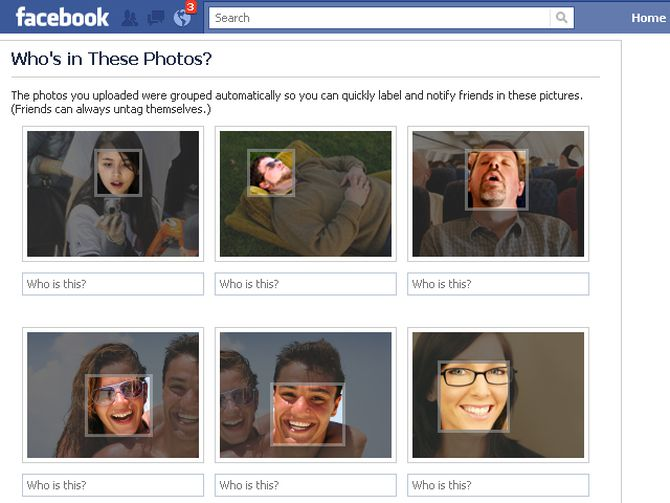
\includegraphics[width=.7\textwidth]{fb}
	\end{figure}
	Face recognition is one of the applications of using intelligent systems.\\
	{\tiny
	\url{https://www.cnet.com/how-to/how-to-disable-facial-recognition-in-facebook/}
	}
\end{frame}

\begin{frame}{Introduction}
	\begin{figure}
		\centering
		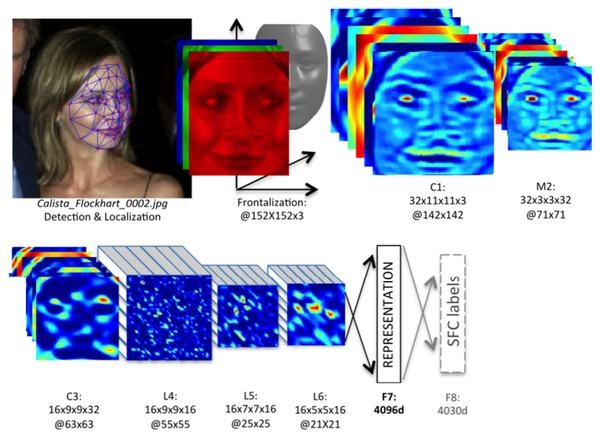
\includegraphics[width=.3\textwidth]{fb2}
		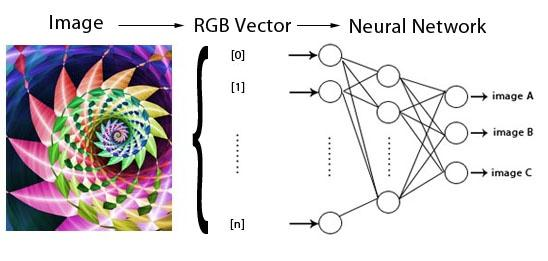
\includegraphics[width=0.45\textwidth]{img1}\\
		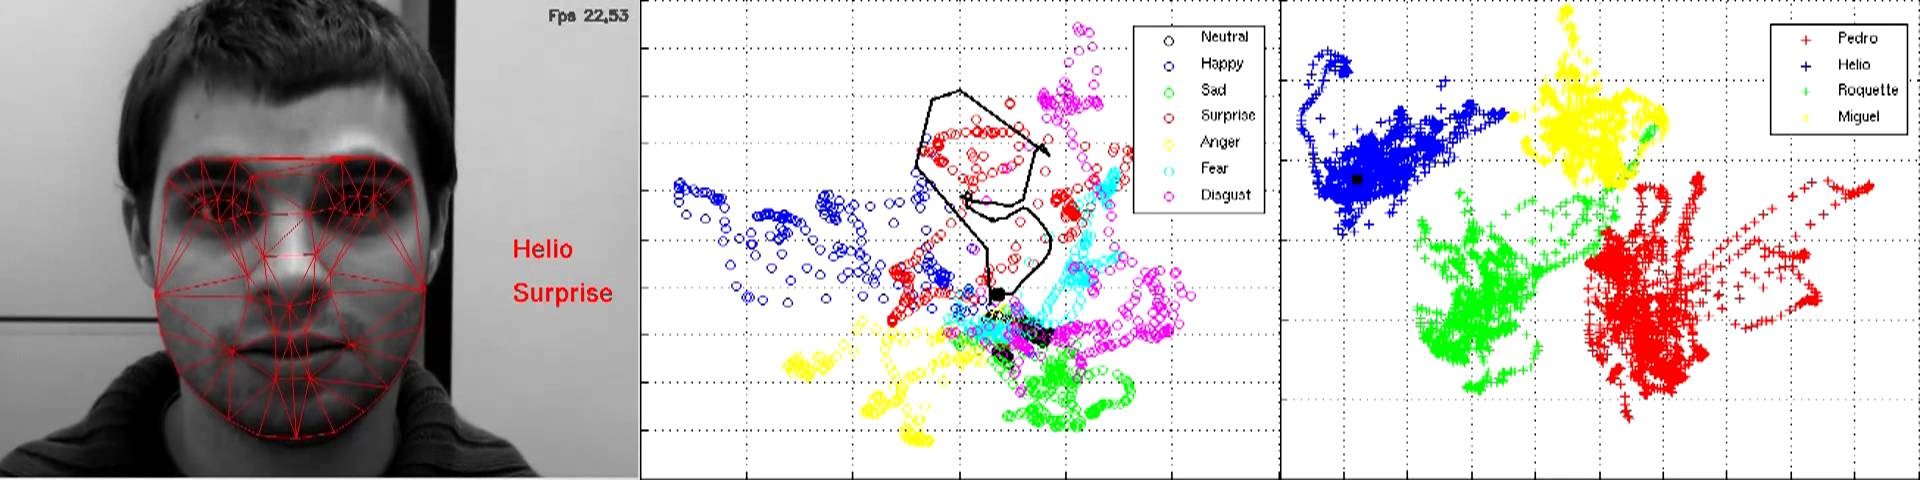
\includegraphics[width=0.8\textwidth]{img2}
	\end{figure}
	{\tiny
	\url{http://neuroph.sourceforge.net/image_recognition.html}\\\url{https://www.grahamcluley.com/facebook-facial-recognition}\\\url{https://www.youtube.com/watch?v=OpioH4v47N0}}
\end{frame}

\section{Problem Statement}
\begin{frame}{Problem Statement}
	\begin{itemize}
		\item<1-> What are the optimal parameters of the best SVM classifier?
		\item<1-> How is the performance of an optimal classifier?
		\item<1-> To recognize people's face with(out) sunglasses
	\end{itemize}
\end{frame}

\section{Methodology}
\begin{frame}{Dataset}
	\begin{figure}
		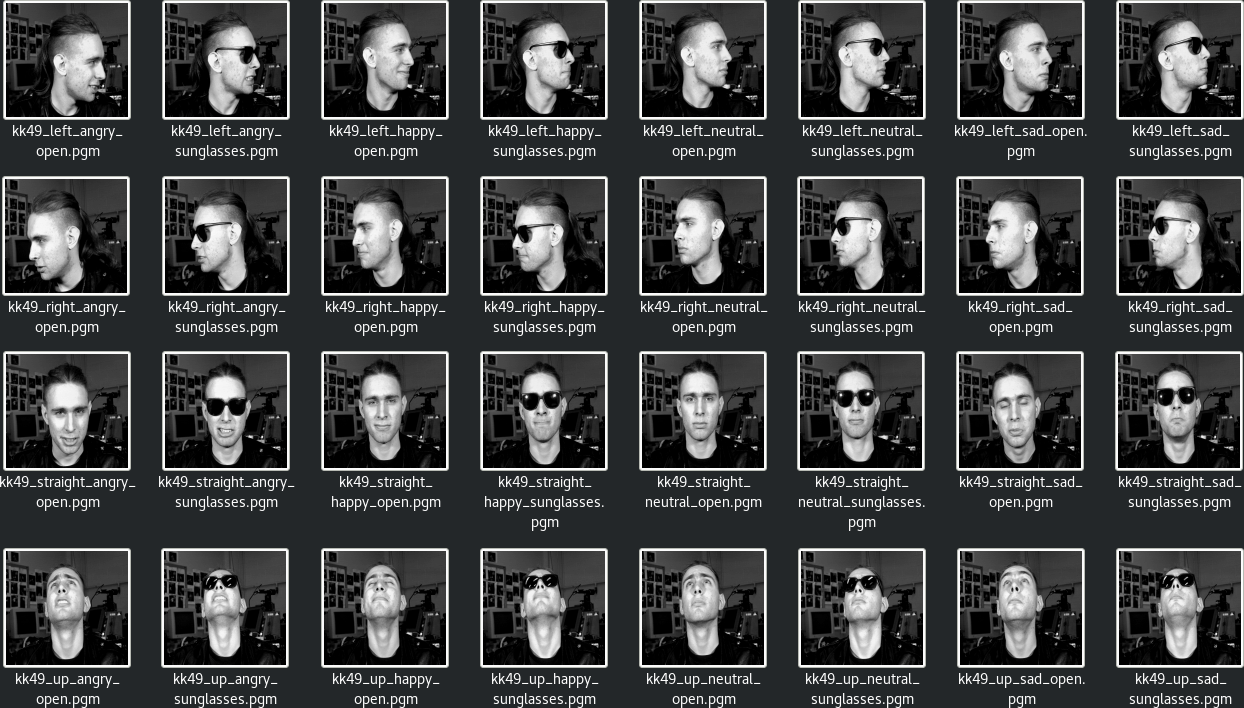
\includegraphics[width=.9\textwidth]{male}
	\end{figure}
	\textit{CMU face images} data set: 20 persons with 16 poses each
\end{frame}

\begin{frame}{Dataset}
	\begin{figure}
		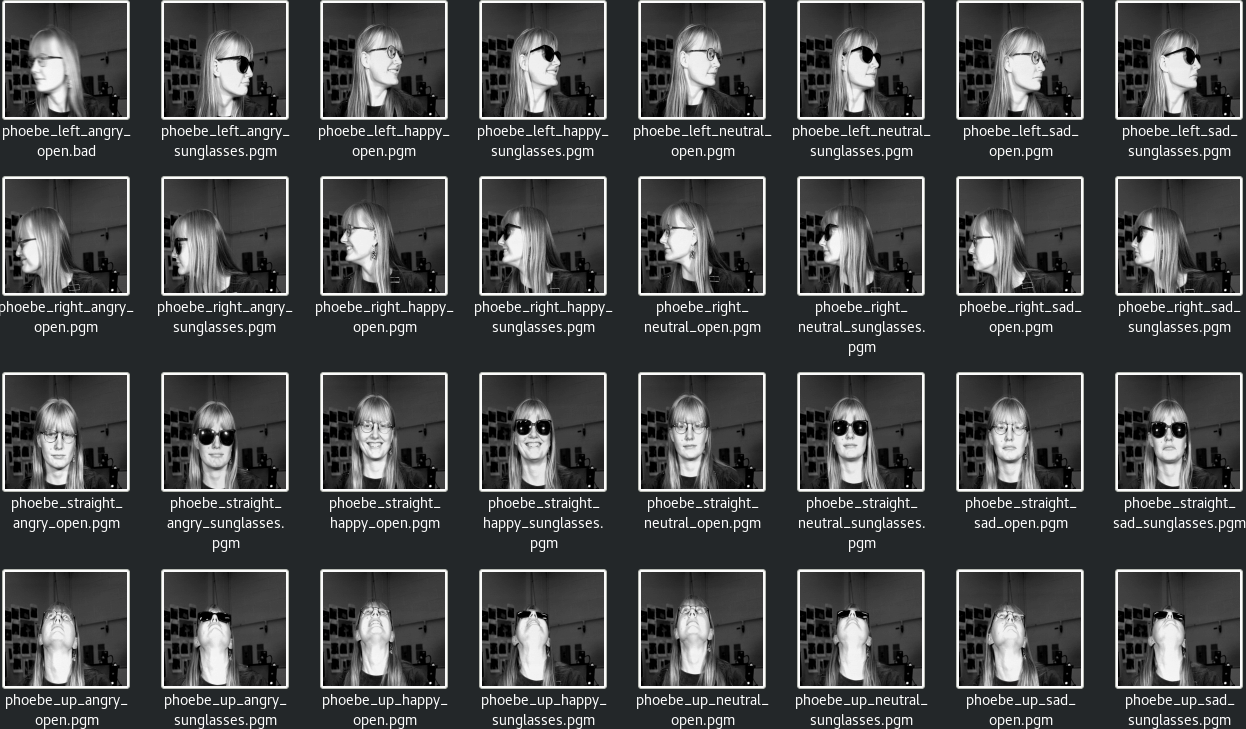
\includegraphics[width=.9\textwidth]{female}
	\end{figure}
	\textit{CMU face images} data set: 20 persons with 16 poses each
\end{frame}

\begin{frame}{Dataset}
	\begin{columns}
		\begin{column}{0.5\textwidth}<1->  %%<--- here
			\begin{center}
				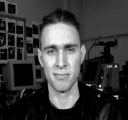
\includegraphics[width=.5\textwidth]{sample}\\
				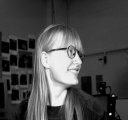
\includegraphics[width=.5\textwidth]{sample1}
			\end{center}
		\end{column}
		\begin{column}{0.5\textwidth}<1->
		PGM image specification\\
		\texttt{P2\\
				24 7\\
				15\\
				0  0  0  0  0  0  0  0  ...\\
				0  3  3  3  3  0  0  7  ...\\
				0  3  0  0  0  0  0  7  ...\\
				0  3  3  3  0  0  0  7  ...\\
				0  3  0  0  0  0  0  7  ...\\
				0  3  0  0  0  0  0  7  ...\\
				0  0  0  0  0  0  0  0  ...\\}
		\end{column}
	\end{columns}
\end{frame}

\begin{frame}{\texttt{scikit-learn}}
	\begin{figure}
		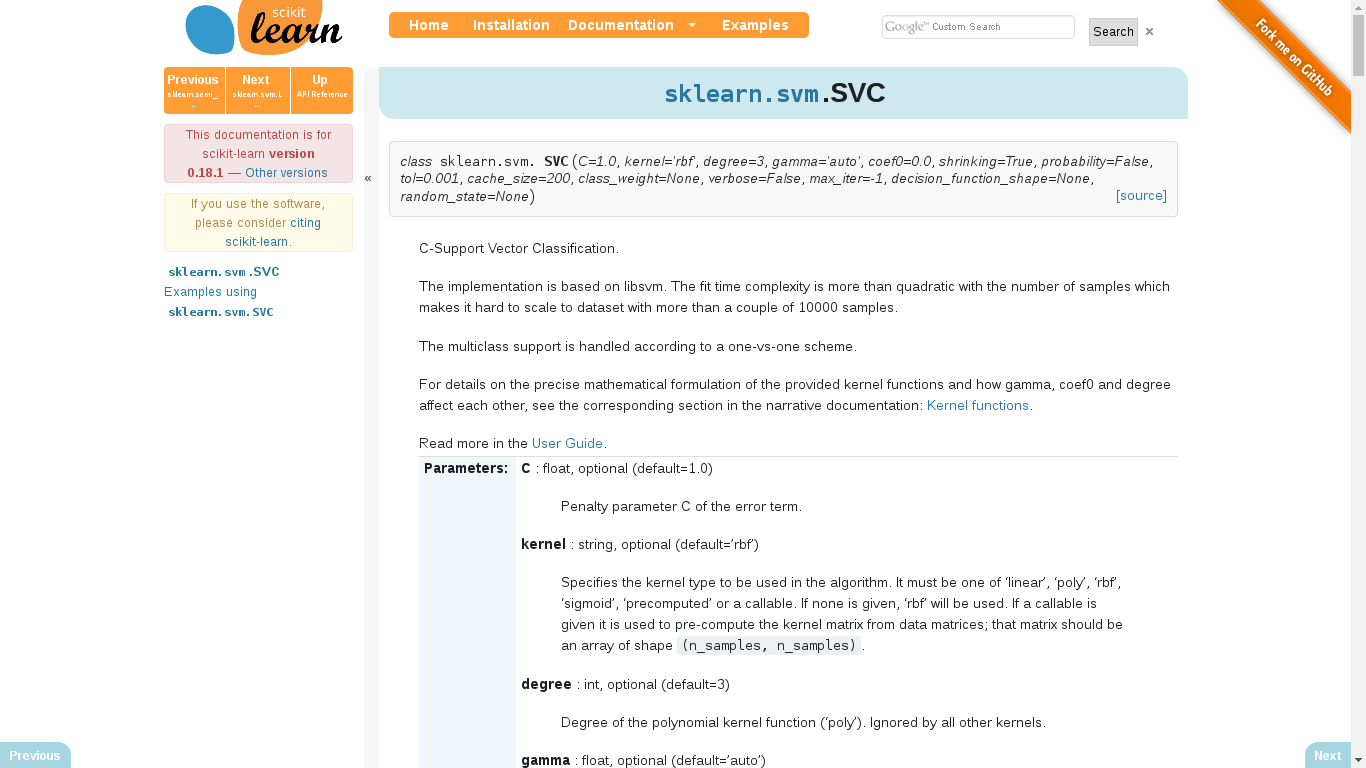
\includegraphics[width=1\textwidth]{svm}
	\end{figure}
\end{frame}

\begin{frame}{\texttt{scikit-learn}}
	\begin{itemize}
		\item<1->  \texttt{gamma} measures how far the influence of a single instance reaches in the multi-dimensional space. \textit{Low values mean 'far'}.
		\item<1->  \texttt{C} trades off misclassification against simplicity of the decision surface. \textit{Low \texttt{C} makes it smooth}.
	\end{itemize}
\end{frame}

\begin{frame}{\texttt{scikit-learn}}
	\begin{figure}
		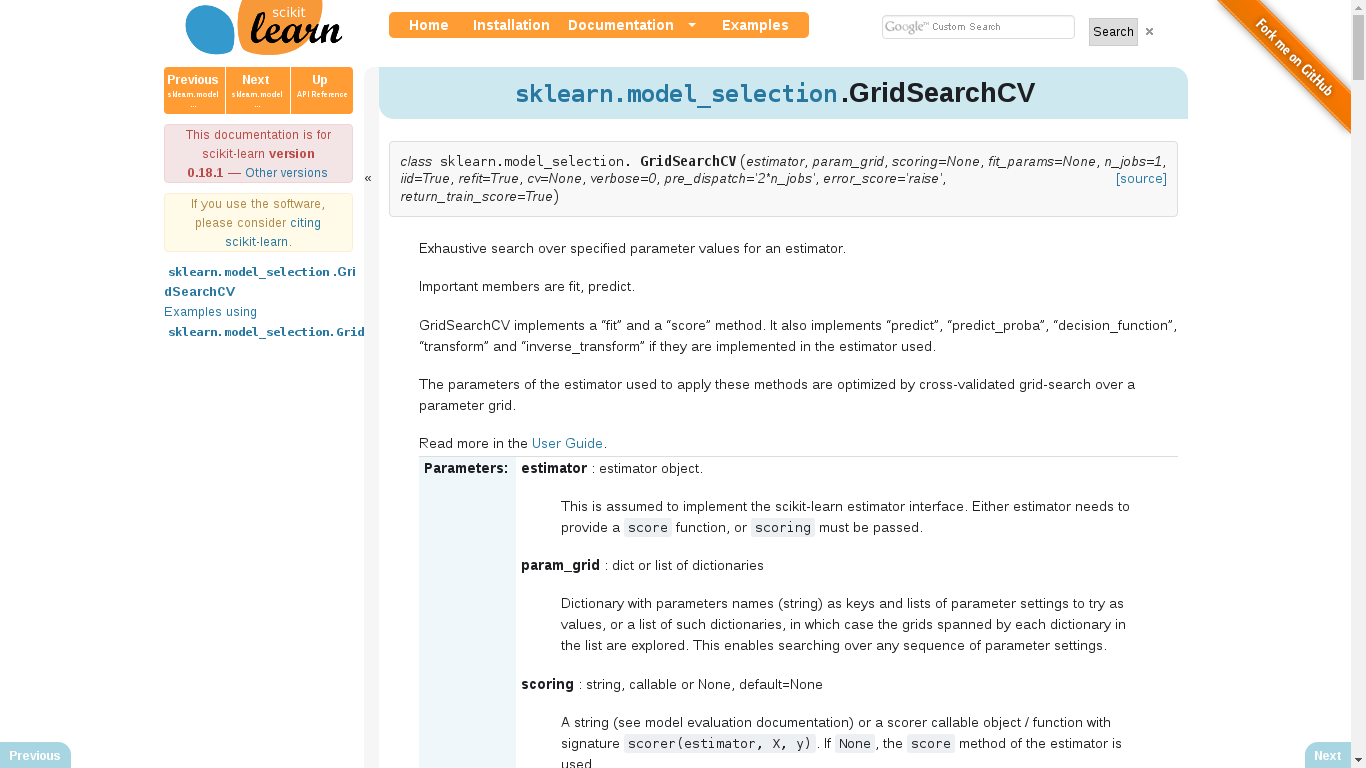
\includegraphics[width=1\textwidth]{gcv}
	\end{figure}
\end{frame}

\begin{frame}{\texttt{scikit-learn}}
	\begin{block}{Why do we use open-source libraries?}
		\begin{itemize}
			\item<1-> More time to analyze the dataset and tuning the parameters instead of implementing the classifier
			\item<1-> Open-source collaboration made the source code more optimized
		\end{itemize}
	\end{block}
\end{frame}

\section{Results}

\begin{frame}{GCV}
	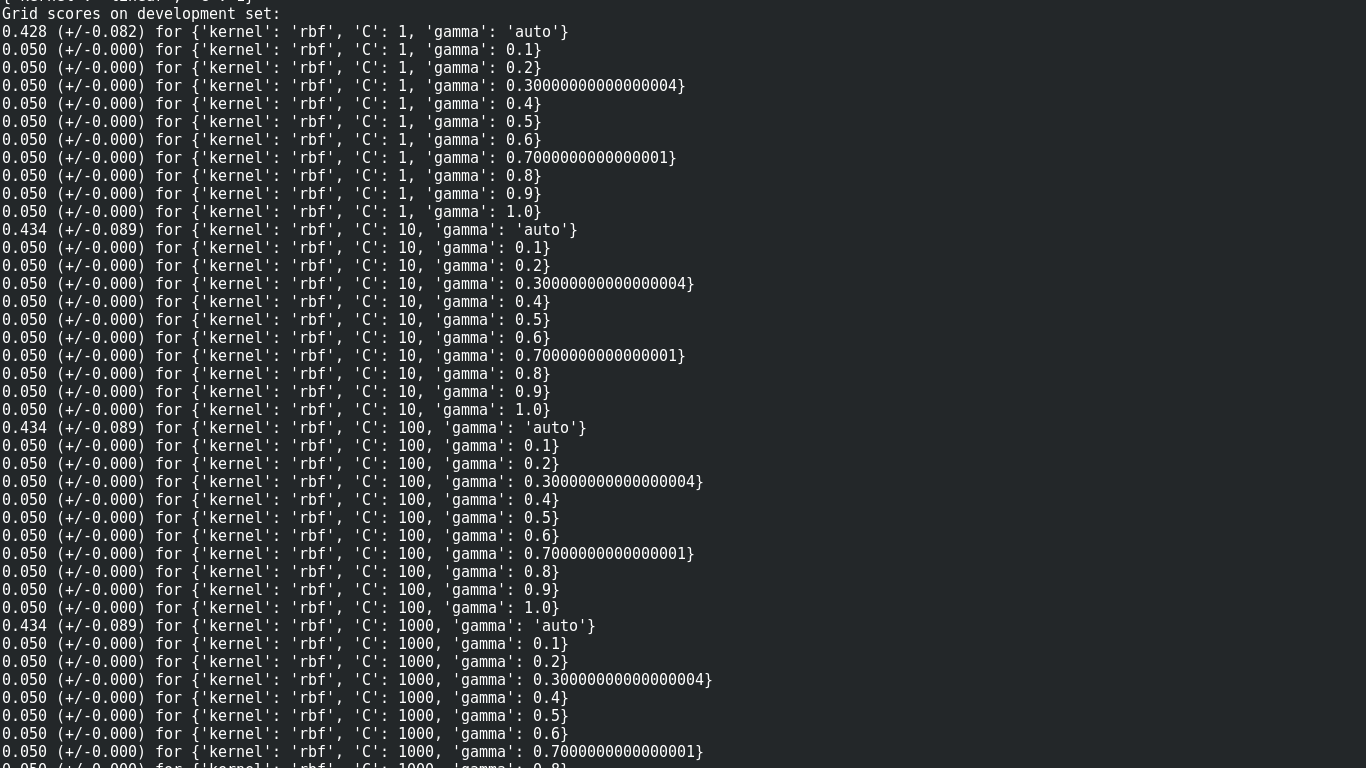
\includegraphics[width=\textwidth]{output}
\end{frame}

\begin{frame}{SVM}
	\begin{figure}
		\centering
		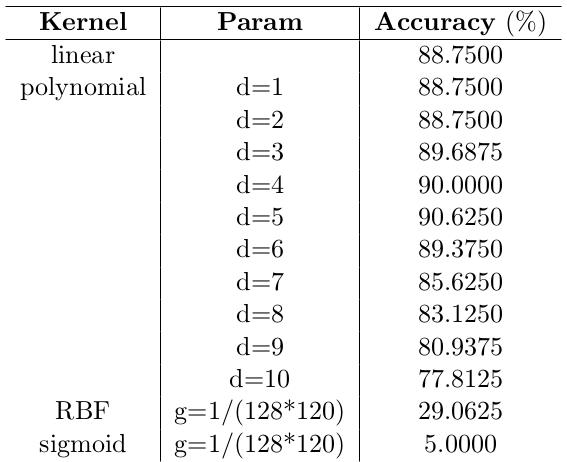
\includegraphics[width=0.5\textwidth]{svmout}
	\end{figure}
	\begin{itemize}
		\item<1-> Accuracy not that sensitive to \texttt{gamma} and \texttt{C}
		\item<1-> Support vectors: 291/320, expected result
	\end{itemize}
\end{frame}

\begin{frame}{Conclusion}
	\begin{itemize}
		\item<1-> SVM with polynomial kernel generally performs better for face recognition problem
		\item<2-> There are so much methods to apply! See PCA, eigenfaces and deep learning
	\end{itemize}
\end{frame}


\end{document}